\documentclass{beamer}

\usepackage{wrapfig}
\usepackage[linesnumbered,ruled,vlined]{algorithm2e}
\usepackage{tikz}
\usepackage{pgfplots}
\usepackage{graphicx}
\pgfplotsset{compat=1.18}
\usepackage{amsmath}
\usetikzlibrary{intersections, through, calc}

\renewcommand{\algorithmcfname}{Algorithmus}

% Theme and colors
\usetheme{Singapore} % Clean layout
\usecolortheme{default}

% Custom colors
\definecolor{DarkBlue}{RGB}{10, 25, 47} % Dark navy
\definecolor{FrameTextColor}{RGB}{255,255,255}

% Set background canvas color (header/footer)
\setbeamercolor{frametitle}{bg=DarkBlue, fg=FrameTextColor}
\setbeamercolor{title}{bg=DarkBlue, fg=FrameTextColor}
\setbeamercolor{author}{fg=FrameTextColor}
\setbeamercolor{date}{fg=FrameTextColor}
\setbeamercolor{section in head/foot}{bg=DarkBlue, fg=FrameTextColor}
\setbeamercolor{subsection in head/foot}{bg=DarkBlue, fg=FrameTextColor}
\setbeamercolor{footline}{bg=DarkBlue, fg=FrameTextColor}
\setbeamercolor{headline}{bg=DarkBlue, fg=FrameTextColor}

% Remove navigation symbols
\setbeamertemplate{navigation symbols}{}

% Title page setup
\title[Kolloquium]{Kolloquium}
\subtitle[Die geometrische Brownsche Bewegung und Anwendungen]{Die geometrische Brownsche Bewegung und Anwendungen}
\author{Fabian Schuller}
\date{\today}

% Custom footline (optional)
\setbeamertemplate{footline}{
  \leavevmode%
  \hbox{%
  \begin{beamercolorbox}[wd=0.7\paperwidth,ht=2.5ex,dp=1ex,left]{author in head/foot}%
    \hspace{1em}\insertshortauthor{} - \insertshorttitle{}
  \end{beamercolorbox}%
  \begin{beamercolorbox}[wd=0.3\paperwidth,ht=2.5ex,dp=1ex,right]{date in head/foot}%
    \insertframenumber{} / \inserttotalframenumber\hspace{1em}
  \end{beamercolorbox}}%
  \vskip0pt%
}

% Begin document
\begin{document}

\section{Einleitung}

\begin{frame}
  \titlepage
\end{frame}

\begin{frame}{Ablauf}
  \begin{itemize}
    \item Presentation der Inhalte der Bachelorarbeit
    \begin{itemize}
      \item Grundlagen zu Stochastischen Prozessen und der Brownschen Bewegung
      \item Motivation der geometrischen Brownschen Bewegung
      \item Modellierung von Finanzzeitreihen mit der geometrischen Brownschen Bewegung
      \item Bewertung von Aktienoptionen mit dem Black-Scholes-Modell
      \item Weiterführende Themen: Stochastische Differentialgleichungen und das CEV-Modell
    \end{itemize}
    \item Diskussion
  \end{itemize}
\end{frame}

\section{Die Brownsche Bewegung}

\begin{frame}{Stochastische Prozesse}
    \begin{itemize}
      \item Folgen bzw. Familien von Zufallsvariablen $$X_t,\quad t \in \Bbb N \quad \mathrm{ bzw. } \quad  t \in \Bbb R_{\ge 0}$$
      \item Zeitdiskrete Prozesse: Wiederholter Münzwurf, Zufallsspaziergang
      \item Zeitstetige Prozesse: Brownsche Bewegung
    \end{itemize}
    \begin{figure}
      \centering
      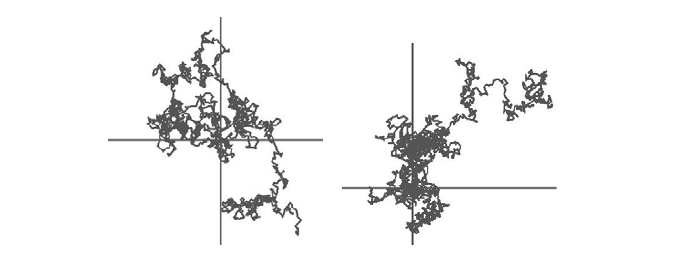
\includegraphics[width=1\textwidth]{images/bb_2d.png}
    \end{figure}
\end{frame}

\begin{frame}{Die diskrete Brownsche Bewegung}
  \begin{itemize}
    \item Konstruktion durch aufsummierte unabhängige Normalvariablen
    \item Skaliertes Interpolationsverfahren (N-ter Ordnung)
  \end{itemize}
  \begin{figure}
    \centering
  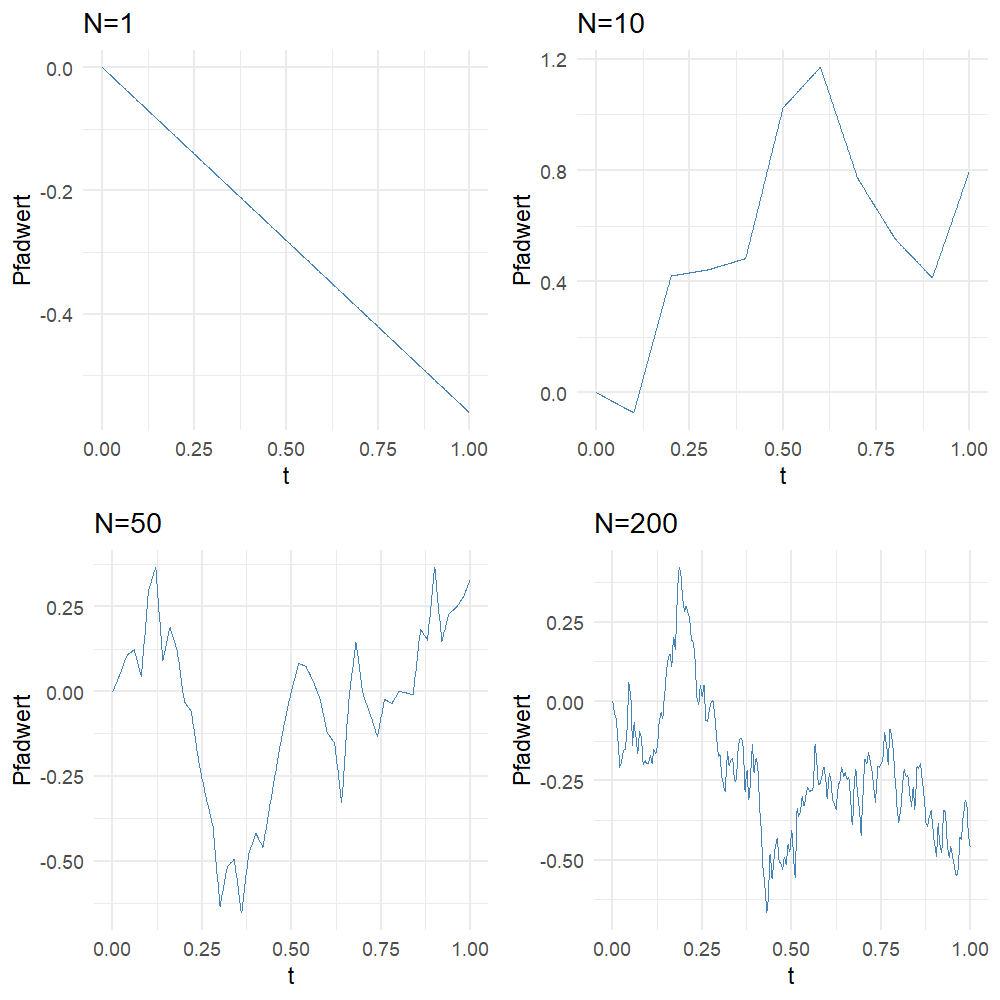
\includegraphics[width=0.55\textwidth]{../thesis/images/disrete_bb.png}
  \end{figure}
\end{frame}

\begin{frame}{Die Brownsche Bewegung}
  \begin{itemize}
  \item Klassische Axiome
    \begin{enumerate}
      \item $W_0=0$ (fast-sicher)
      \item Die Pfade $t \mapsto W_t$ sind (fast-sicher) stetig
      \item Für Zeitpunkte $0 \le t_0 < t_1 \dots$ sind die Zuwächse $W_{t_1} - W_{t_0}$ unabhängig
      \item Die Zuwächse sind normalverteilt mit $W_{t_1} - W_{t_0} \sim N(0, t_1 - t_0)$
    \end{enumerate}
  \pause
  \item Brownsche Bewegung als Grenzwert
    \begin{itemize}
      \item Diskrete Brownsche Bewegung und dann $N \to \infty$
      \item Um die Axiome Nachzuweisen und Verteilungskonvergenz im Funktionenraum: Satz von Donsker
      \item In der Arbeit: Existenz der endlich-dimensionalen Verteilungen (mit Cramér-Wold) und Nachweis der Stetigkeit
    \end{itemize}
\end{itemize}
\end{frame}

\begin{frame}{Kovarianzstruktur der Brownschen Bewegung}
  \begin{itemize}
    \item Kovarianz: $\mathrm{Cov}(W_s,W_t)=\min(s,t)$
    \item Bedingte Verteilung: $W_t \mid W_s \sim \mathcal N(W_s,\, t-s)$
  \end{itemize}
  \begin{figure}
    \centering
  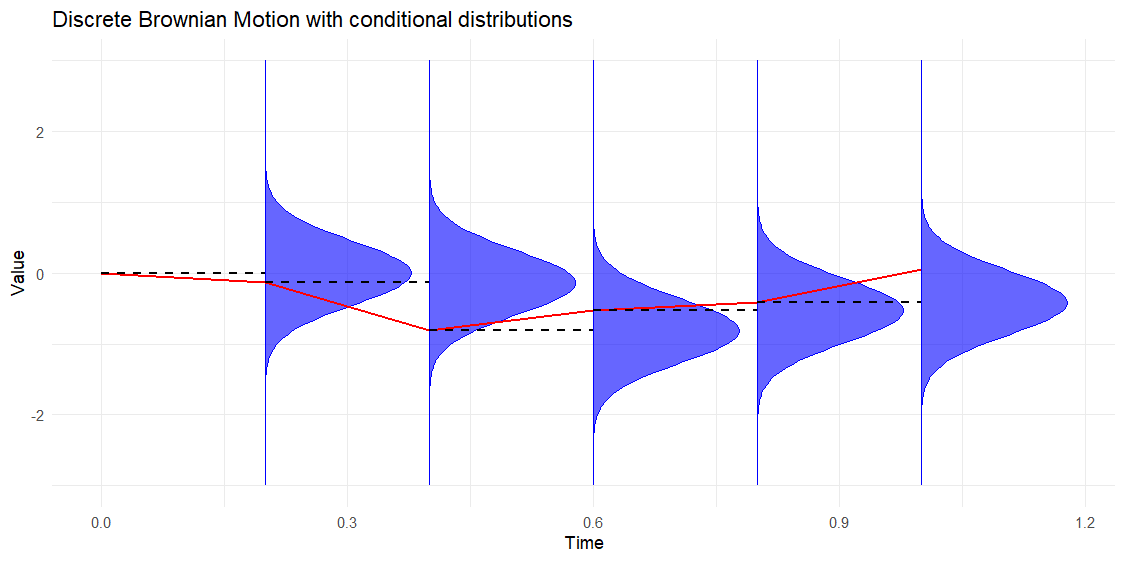
\includegraphics[width=0.88\textwidth]{../thesis/images/bb_with_cov_wide.png}
  \end{figure}
\end{frame}

\begin{frame}{Eigenschaften der Brownschen Bewegung}
  \begin{itemize}
      \item Martingal-Eigenschaft
      \begin{itemize}
        \item $E(W_t | W_s = v) = v$ bzw. $E(W_t | W_s) = W_s$
        \item folgt aus der bedingten Verteilung
      \end{itemize}
      \item Stationäre, unabhängige Inkremente, normalverteilt
      \item Pfade sind stetig aber nicht differenzierbar (fast-sicher)
      \item Somit eignet sich die Brownsche Bewegung zur Modellierung von Rauschen (Zufälliges Element in einem Prozess)
  \end{itemize}
\end{frame}

\section{Die geometrische Brownsche Bewegung}

\begin{frame}{Die geometrische Brownsche Bewegung}
  \begin{itemize}
      \item Multiplikatives Modell: $S_{k+1}=S_k(1+X_{k+1})$
      \item Annahme: $X_{k+1}=\mu\Delta t+\sigma\sqrt{\Delta t}\,\varepsilon_{k+1}$
      \item $\varepsilon_k$ i.i.d mit $E(\varepsilon_k)=0$, $V(\varepsilon_k)=1$. (Z. B. $\mathcal N(0,1)$-Verteilt)
      \item Dies kann man als diskrete stochastische Differenzengleichung (SDE) interpretieren.
      \item Genauer: Euler-Maruyama-Approximation der SDE $$dS_t = \mu S_t\,dt + \sigma S_t\,dW_t$$
  \end{itemize}
\end{frame}

\begin{frame}{Geschlossene Formel}
  \begin{itemize}
      \item Geschlossene Lösung der SDE / Grenzwert der diskreten Übergangsvariablen
      \begin{itemize}
        \item Limes: $\Delta t \to 0$ (Zeit-Schritt) und $n \to \infty$ (Anzahl der Messungen)
      \end{itemize}
      \item $S_T = S_0 \exp\big((\mu-\tfrac12\sigma^2)T + \sigma W_T\big)$
      \item $S_T$ ist log-normalverteilt
  \end{itemize}
\end{frame}

\begin{frame}{Beweisskizze}
  \begin{itemize}
      \item Ausgangspunkt: $S_{k+1}=S_k(1+X_{k+1})$ mit $X_{k+1}=\mu\Delta t+\sigma\sqrt{\Delta t}\,\varepsilon_{k+1}$
      \item Logarithmierung: $\log S_n = \log S_0 + \sum \log(1+X_j)$
      \item Taylor-Entwicklung bis 2. Ordnung, danach $$
\begin{aligned}
\log S_n &\approx \log S_0 + \sum_{j=1}^n\left( \underbrace{\mu \Delta t + \sigma\sqrt{\Delta t} \varepsilon_j}_{X_j} - \underbrace{\frac{1}{2} \sigma^2 \Delta t \varepsilon_j}_{-\frac{1}{2} X_j^2} \right)
\\ &= \log S_0 + \mu T +  \underbrace{\sigma\sqrt{\Delta t} \sum_{j=1}^{n} \varepsilon_j}_{\mathrm{[ZGWS]} \quad \to \sigma W_T} - \underbrace{\frac{1}{2} \sigma^2 \sum_{j=1}^{n} \Delta t \varepsilon_j^2}_{\mathrm{[GGZ]} \quad \to \frac12 \sigma^2 T}
\end{aligned}
$$
      \item Letztlich $\log S_T \overset{d} = \log S_0 + \big(\mu - \tfrac12 \sigma^2\big)T + \sigma W_T$ \qed
  \end{itemize}
\end{frame}

\begin{frame}{Fazit und Eigenschaften}
  \begin{itemize}
      \item Positivität: $S_t>0$ fast sicher
      \item fast sicher stetige Pfade
      \item Log-Normalverteilt mit $\log S_t \sim N(\log S_0 + (\mu - \tfrac12 \sigma^2)t, \sigma^2 t)$
  \end{itemize}
\end{frame}

\section{Anwendungen}

\begin{frame}{Kalibrierung}
  \begin{itemize}
      \item Schätzung von $\mu,\sigma$ über Log-Returns
      \begin{itemize}
        \item Daten sind zu einem festen $\Delta t$ gegeben
        \item Aus $\log S_{t + \Delta t} - \log S_t \sim \mathcal N((\mu - \tfrac12 \sigma^2)\Delta t, \sqrt{\sigma} \Delta t)$ folgt der Schätzer
        \item $\sigma^2 = s^2(\Delta \log S_t) / \Delta t$ und $\mu = m(\Delta \log S_t) / \Delta t + \tfrac12 \sigma^2$ wobei $s^2$ die empirische Varianz und $m$ das Mittel ist
      \end{itemize}
      \pause
      \item Konfidenzintervalle und Unsicherheitsschätzung (Bootstrap)
      \begin{itemize}
        \item Die Daten sind ggf. unrein
        \item Schätze $\mu$ und $\sigma$ wiederholt aus einer Teilmenge der Daten schätzt
        \item Resultat ist ein Konfidenzintervall für $\mu$ und $\sigma$
      \end{itemize}
  \end{itemize}
\end{frame}

\begin{frame}{Simulation}
  \begin{itemize}
      \item Exakte Pfadsimulation für GBM mit der geschlossenen Formel und der diskreten Brownsche Bewegung
      \item Anwendung z. B. Monte-Carlo-Simulation für Optionspreise
      \item Numerik: Euler-Maruyama für verallgemeinerte Modelle (CEV etc.)
  \end{itemize}
  \begin{figure}
    \centering
  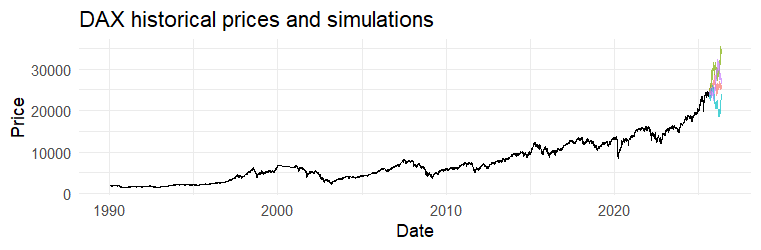
\includegraphics[width=0.88\textwidth]{../thesis/images/dax_monte_carlo.png}
  \end{figure}
\end{frame}

\begin{frame}{Backtests}
  \begin{itemize}
      \item Validierung eines Modells anhand historischer Daten
      \item Metriken zur Bewertung
  
  \end{itemize}
\begin{table}[H]
\centering
\begin{tabular}{lcccccc}
Hitratio & MSE \\

\% im Konfidenzintervall & $\frac{1}{n} \sum_{i=1}^n (y_i - \hat{y}_i)^2$  \\
\hline
NRMSE & MAPE \\
$\frac{\sqrt{\text{MSE}}}{y_{max} - y_{min}}$ & $\frac{100\%}{n} \sum_{i=1}^n \left|\frac{y_i - \hat{y}_i}{y_i}\right|$ \\

\end{tabular}
\end{table}

\end{frame}

\begin{frame}{Visualisierung von Backtests}
  \begin{figure}
    \centering
  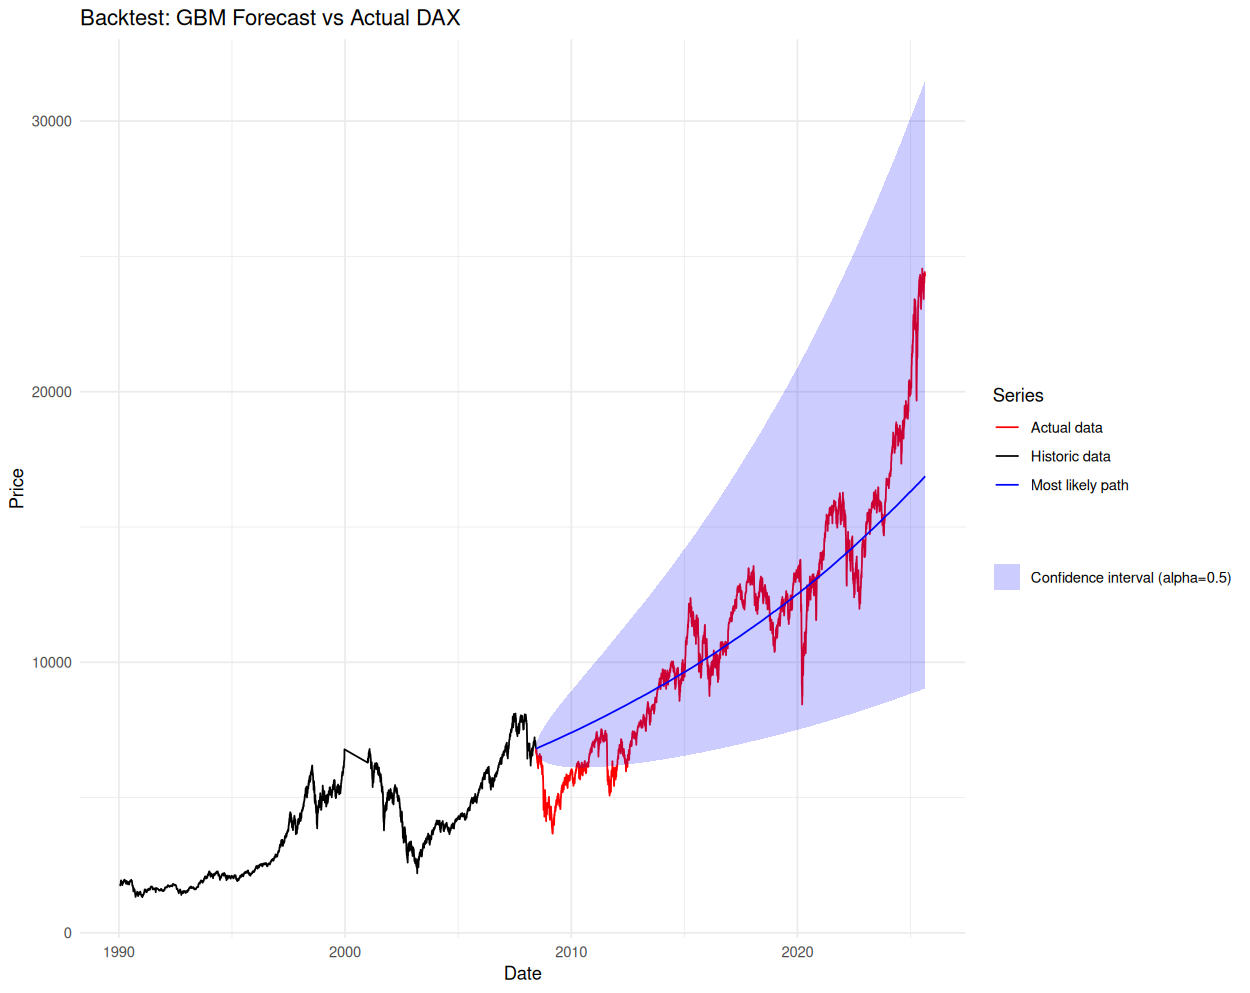
\includegraphics[width=0.49\textwidth]{../thesis/images/dax_backtest.png}
  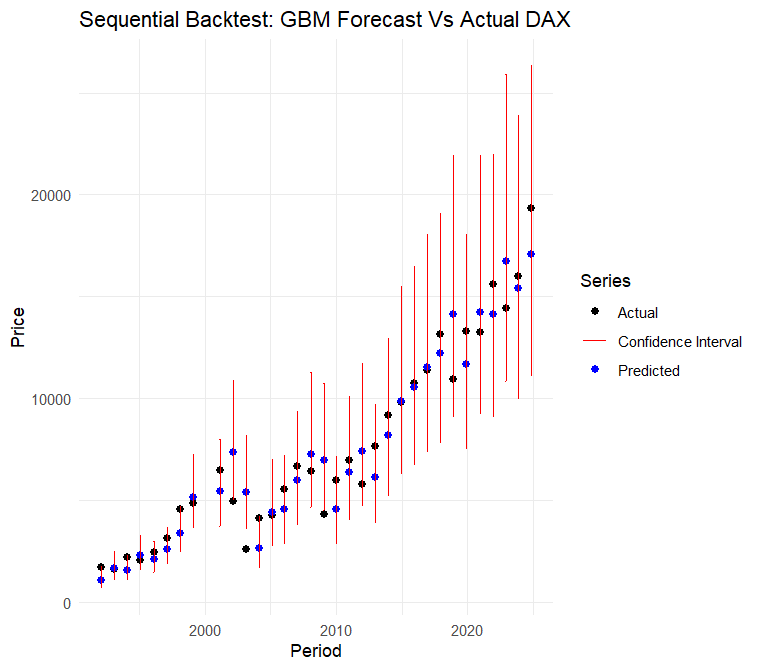
\includegraphics[width=0.49\textwidth]{../thesis/images/dax_backtest_seq.png}
  \end{figure}
\end{frame}

\section{Black-Scholes}

\begin{frame}{Optionen}
  \begin{itemize}
      \item Eine europäische Call Option gibt dem Käufer das Recht, aber nicht die Pflicht, eine Aktie am Zeitpunkt $T$ zum Ausübungspreis $K$ zu kaufen.
      \item Put Option: Recht auf Verkauf (an den Anbieter der Option)
      \begin{itemize}
        \item Beispiel: Absicherung von Getreide-Ernte
      \end{itemize} 
      \item Auszahlungsfunktion $\max(S_T-K,0)$ (Call), $\max(K-S_T, 0)$ (Put)
      \item Es gibt viele weitere Optionstypen mit anderen Auszahlungen
  \end{itemize}
\end{frame}

\begin{frame}{Bewertung von Optionen}
  \begin{itemize}
      \item Naiver Ansatz: Erwartungswert der Ausübungsfunktion unter einem Aktienkursmodell wie der GBM
      \pause
      \item Was ist mehr Wert? 100€ jetzt oder 100€ in einem Jahr?
      \pause
      \item 100€ jetzt, denn man könnte das Geld anlegen, und 2\% Zinsen erhalten
      \item Modellerweiterung: Bank bietet risikofreien Zinssatz $r$
  \end{itemize}
\end{frame}

\begin{frame}{Black-Scholes Modell}
  \begin{itemize}
      \item Im Black-Scholes Modell wird der Wert der Option durch eine GBM modelliert
      \begin{itemize}
        \item Der Diffusionsterm bleibt $\sigma$, wie bei der Aktie
        \item Als Drift-Term setzt man den risiko-neutralen Zinsatz $r$
      \end{itemize}
      \item Black-Scholes Modell wird eine risiko-neutrale Welt angenommen, da man die Risikopräferenzen der Anleger nicht kennt
  \end{itemize}
\end{frame}

\begin{frame}{Risikoneutrale Bewertung von Optionen}
  \begin{itemize}
      \item Der risikofreie Kurs kann nun keinen größeren Erwartungswert haben als das Bankkonto, sonst würde niemand bei der Bank Geld anlegen
      \item In der physikalischen Welt hat die Bank den Vorteil, dass die Zinsen garantiert sind. In der risiko-neutralen Welt besteht dieser Vorteil nicht 
      \pause
      \item Die Zins-Erwartung wird ausgleicht (der Kurs diskontiert) $\tilde S_t = e^{-r t} S_t$
      \item Der diskontierte Kurs (in der risiko-freien-Welt) den Erwartungswert $0$, sogar:
      \item Die Martingal-Eigenschaft: für $s < t$ gilt $$E(e^{-rt}S_t | S_s = v) = e^{-rs} v$$
      \pause
      \item Man konstruiert das risikoneutrale Maß $Q$, um die Martingaleigenschaft des diskontierten Kurses zu garantieren, und nutzt dieses zur Bewertung der Option
  \end{itemize}
\end{frame}


\begin{frame}{Fazit Black-Scholes Modell}
  \begin{itemize}
      \item Modellannahmen: GBM, konstante $r,\sigma$, keine Transaktionskosten
      \item In der Arbeit wird das Black-Scholes Modell als Grenzwert des Binomialmodells hergeleitet
      \item Für europäische Optionen gilt darüber hinaus die explizite Formel
      $$C_0^{\mathrm{BS}}= S_0\,\Phi(d_1) - K e^{-rT}\,\Phi(d_2)$$ mit
      $$
d_1 = \frac{\ln(S_0/K) + \big(r + \tfrac12 \sigma^2\big)T}{\sigma \sqrt{T}},
\qquad
d_2 = d_1 - \sigma \sqrt{T}.
$$
  \end{itemize}
\end{frame}

\begin{frame}{Beispiele}
  \begin{itemize}
      \item Numerische Bewertung vs. geschlossene Formel: Vergleich für DAX-Calls
      \item Monte-Carlo- vs. Black-Scholes-Ergebnisvergleiche
  \end{itemize}
  \begin{figure}
    \centering
  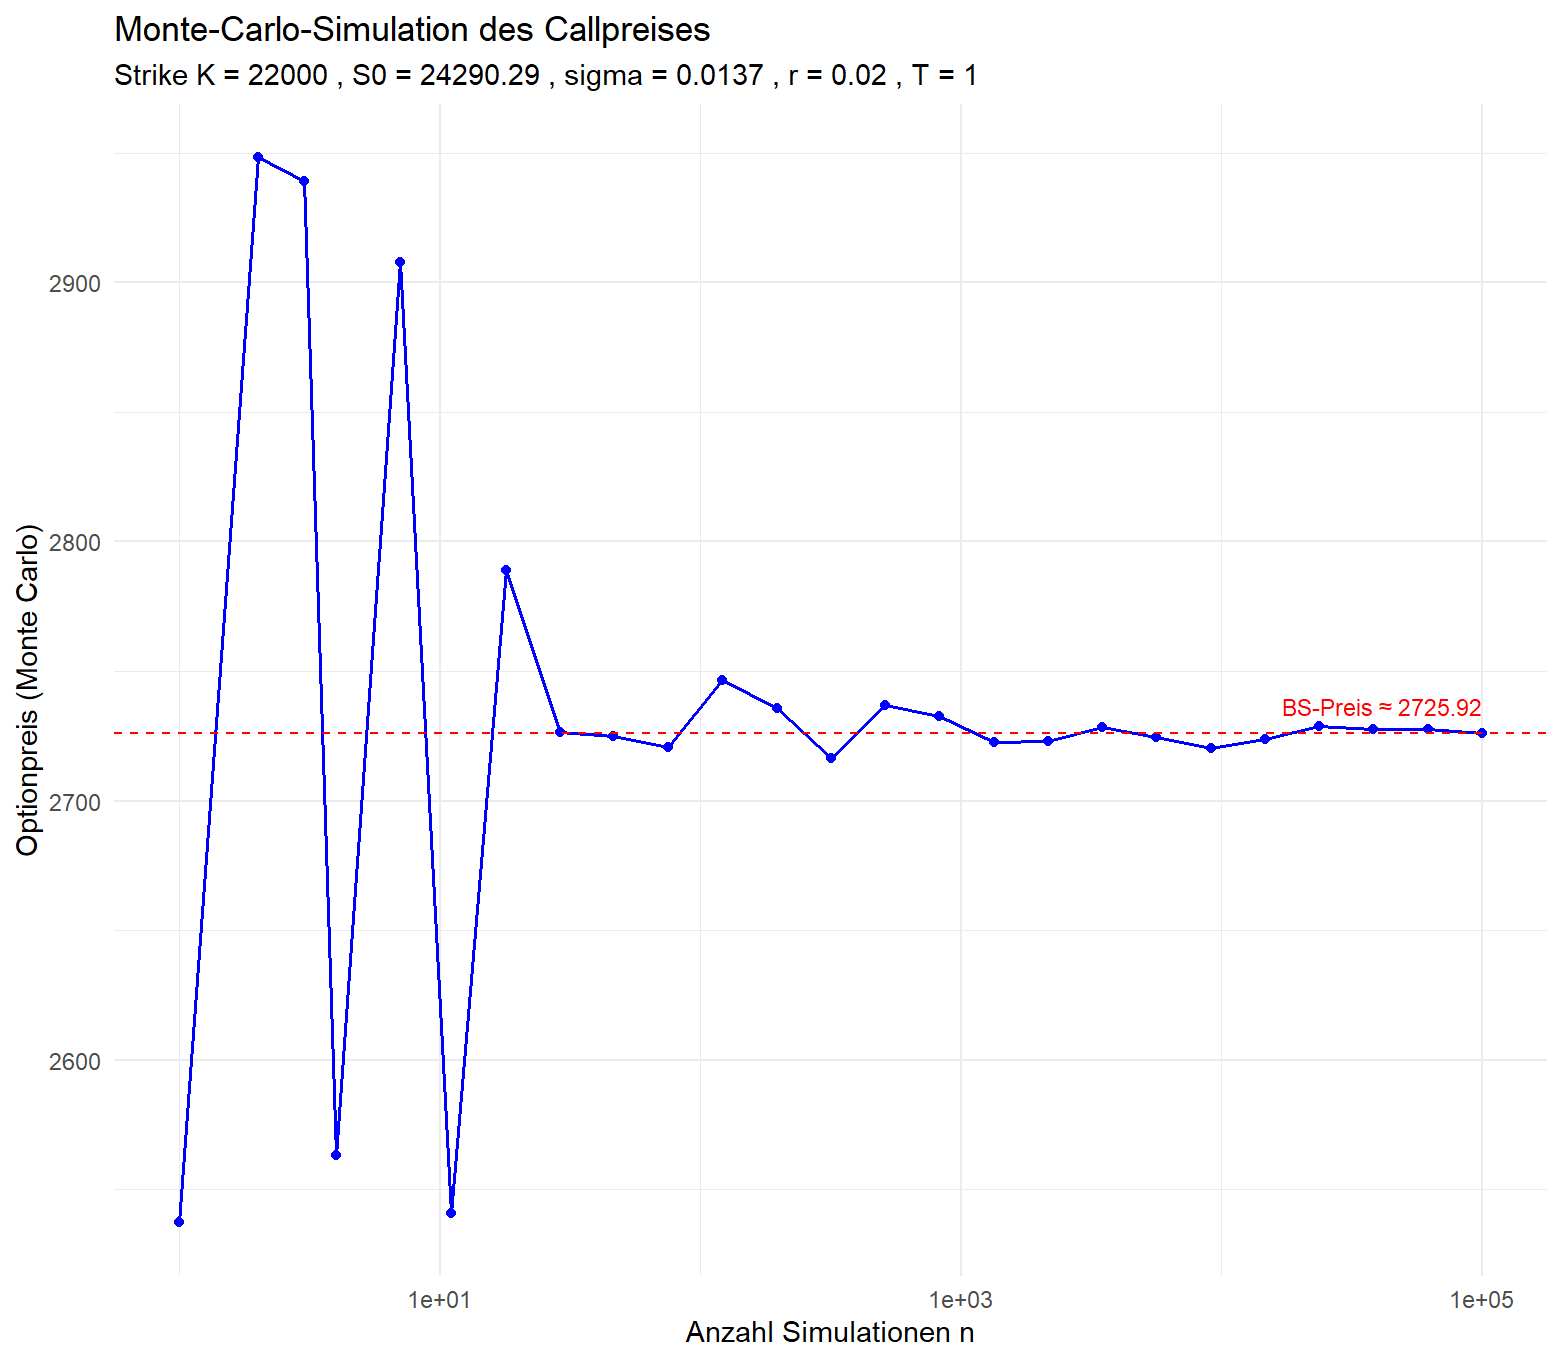
\includegraphics[width=0.88\textwidth]{../thesis/images/call_dax_mc.png}
  \end{figure}
\end{frame}

\section{Ausblick}

\begin{frame}{Stochastische Differentialgleichungen}
  \begin{itemize}
    \item Die Brownsche Bewegung ist (fast-sicher) nicht differenzierbar, dennoch möchte man zeit-stetige Zeitreihen durch DGLs modellieren
    \item Differentialgleichungen werden als Integralgleichung interpretiert
    $$dS_t \;=\; a(S_t,t)\,dt \;+\; b(S_t,t)\,dW_t
$$
wird zu
$$
S_t \;=\; S_0 \;+\; \int_0^t a(S_s,s)\,ds \;+\; \int_0^t b(S_s,s)\,dW_s.
$$
  \item $\int_0^t b(S_s,s)\,dW_s$ heißt It\^o-Integral
  \item Stochastische Integrale werden durch Folgen von "Treppenfunktionen" konstruiert
  \end{itemize}
\end{frame}

\begin{frame}{CEV-Modell}
  \begin{itemize}
    \item Alternative zur GBM
    \item Stochastische Differentialgleichung: $$dS_t \;=\; \mu S_t\,dt \;+\; \sigma\,S_t^{\beta}\,dW_t$$
    \item Diskretisierung: $$\Delta S_i := S_{t_{i+1}} - S_{t_i} \approx \mu S_{t_i}\Delta t + \sigma S_{t_i}^{\beta}\sqrt{\Delta t}\,\varepsilon_i,\quad \varepsilon_i\sim\mathcal N(0,1)$$
    \item Übergangswahrscheinlichkeit: $$\Delta S_i \mid S_{t_i} \sim \mathcal N\left(\mu S_{t_i} \Delta t,\, \sigma^2 S_{t_i}^{2\beta} \Delta t\right)$$
  \end{itemize}
\end{frame}

\begin{frame}{Kalibrierung des CEV-Modell}
  \begin{itemize}
    \item Übergangswahrscheinlichkeit: $$\Delta S_i \mid S_{t_i} \sim \mathcal N\left(\mu S_{t_i} \Delta t,\, \sigma^2 S_{t_i}^{2\beta} \Delta t\right)$$
    \item Dichte: $$p(x) = \frac{1}{\sqrt{2\pi v}} \exp\left(-\frac{(x-m)^2}{2v}\right),\quad m = \mu S_{t_i}, v = \sigma^2 S_{t_i}^{2 \beta}, x=\Delta S_i$$
    \item ML-Schätzer: Betrachte alle Realisierungen der Zeitreihe, und maximiere die Dichte in Abhängigkeit der Parameter
  $$L(\mu, \sigma, \beta) = \prod_{i=0}^{n-1} p(\Delta S_i \mid S_{t_i})$$
    \item Dies wurde in der Arbeit implementiert und mit der GBM verglichen
  \end{itemize}
\end{frame}

\begin{frame}{Schlusswort}
  \centering
  \Huge Vielen Dank für Ihre Aufmerksamkeit\\
\end{frame}

\end{document}